\chapter{开发背景介绍}
\label{chap:2}

\section[MapReduce简介]{MapReduce简介\cite{paper:Google-MapReduce}}
\subsection{MapReduce简介}
Google的很多程序员为了处理海量的原始数据,已经实现了数以百计的、专用的计算方法。这些计算方法用来处理大量的原始数据,比如,文档抓取(类似网络爬虫的程序)、Web请求日志等等;也为了计算处理各种类型的衍生数据,比如倒排索引、Web文档的图结构的各种表示形势、每台主机上网络爬虫抓取的页面数量的汇总、每天被请求的最多的查询的集合等等。大多数这样的数据处理运算在概念上很容易理解。然而由于输入的数据量巨大,因此要想在可接受的时间内完成运算,只有将这些计算分布在成百上千的主机上。如何处理并行计算、如何分发数据、如何处理错误?所有这些问题综合在一起,需要大量的代码处理,因此也使得原本简单的运算变得难以处理。

为了解决上述复杂的问题,Google设计了一个新的抽象模型,使用这个抽象模型,我们只要表述我们想要执行的简单运算即可,而不必关心并行计算、容错、数据分布、负载均衡等复杂的细节,这些问题都被封装在了一个库里面。设计这个抽象模型的灵感来自Lisp和许多其他函数式语言的Map和Reduce的原语。我们意识到我们大多数的运算都包含这样的操作:在输入数据的“逻辑”记录上应用Map操作得出一个中间key/value pair集合,然后在所有具有相同key值的value值上应用Reduce操作,从而达到合并中间的数据,得到一个想要的结果的目的。使用MapReduce模型,再结合用户实现的Map和Reduce函数,用户可以非常容易的实现大规模并行化计算;通过MapReduce模型自带的“再次执行”(re-execution)功能,也提供了初级的容灾实现方案。Google将这种抽象模型做以总结,并于2004在OSDI国际会议上提出\cite{paper:Google-MapReduce},最终风靡全球。

以MapReduce为模型编写的程序能自动地在大规模的普通机器上实现并行化处理。这个系统在运行时需要关注的细节有:分割输入数据,在机群上的调度,机器的错误处理,管理机器之间必要的通信。这样就可以让那些没有并行分布式处理系统经验的程序员使用大量分布式系统的资源。MapReduce可以灵活调整,使其在由普通机器组成的机群上实现运行:一个典型的MapReduce可以计算处理几千台机器上的以TB计算的数据。程序员发现这个系统非常好用:已经实现了数以百计的MapReduce程序,每天在Google的机群上都有1000多个MapReduce程序在执行。

\subsection{MapReduce的实现过程}
MapReduce的实现过程并不复杂,图\ref{fig:MapReduce}向我们展示了MapReduce操作的全部流程。
\begin{figure}[h]
 \centering
 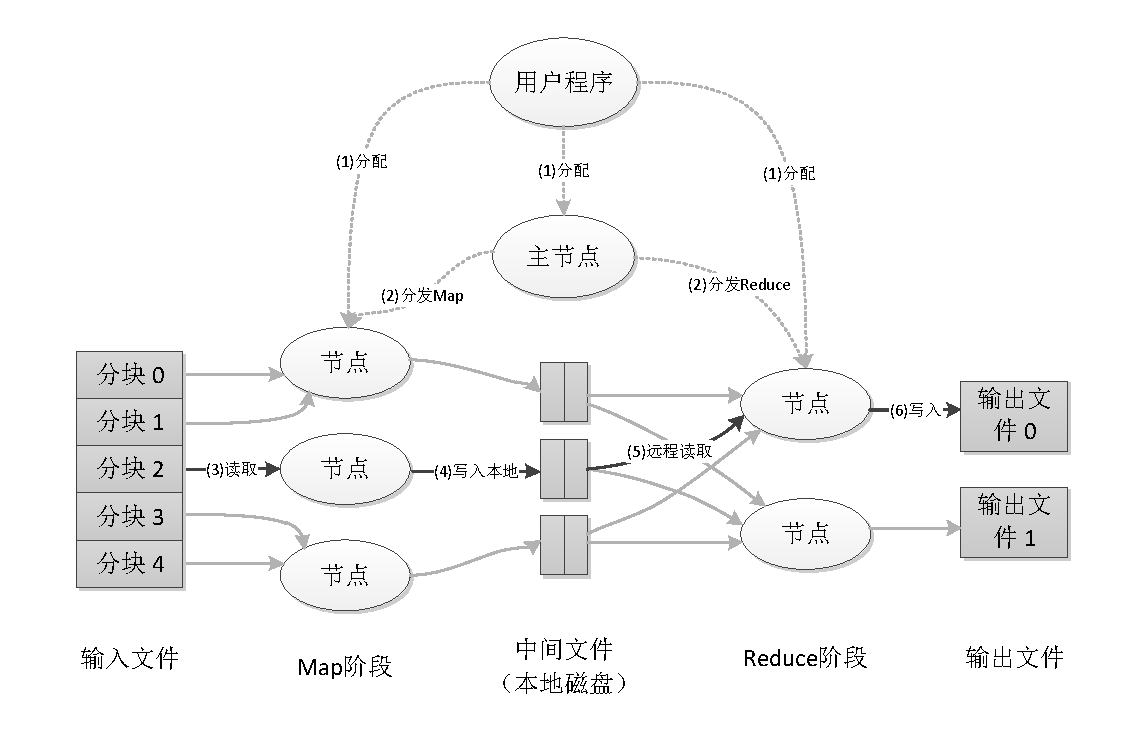
\includegraphics[width=1\textwidth]{MapReduce}
 \caption{MapReduce实现过程}
 \label{fig:MapReduce}
\end{figure}

当用户的程序调用MapReduce的函数的时候,将发生下面的一系列动作(下面的数字和图\ref{fig:MapReduce}中的数字标签相对应):

\begin{enumerate}
\item 在用户程序里的MapReduce库首先分割输入文件成M个片,每个片的大小一般从16到64MB(用户可以通过可选的参数来控制)。然后在机群中开始大量的拷贝程序。

\item 这些程序拷贝中的一个是master,其他的都是由master分配任务的worker。有M个map任务和R个reduce任务将被分配。管理者分配一个map任务或reduce任务给一个空闲的worker。

\item 一个被分配了map任务的worker读取相关输入split的内容。它从输入数据中分析出key/value对,然后把key/value对传递给用户自定义的map函数。由map函数产生的中间key/value对被缓存在内存中。

\item 缓存在内存中的key/value对被周期性的写入到本地磁盘上,通过分割函数把它们写入R个区域。在本地磁盘上的缓存对的位置被传送给master,master负责把这些位置传送给reduce worker。

\item 当一个reduce worker得到master的位置通知的时候,它使用远程过程调用来从map worker的磁盘上读取缓存的数据。当reduce worker读取了所有的中间数据后,它通过排序使具有相同key的内容聚合在一起。因为许多不同的key映射到相同的reduce任务,所以排序是必须的。如果中间数据比内存还大,那么还需要一个外部排序。

\item reduce worker迭代排过序的中间数据,对于遇到的每一个唯一的中间key,它把key和相关的中间value集传递给用户自定义的reduce函数。reduce函数的输出被添加到这个reduce分割的最终的输出文件中。

\item 当所有的map和reduce任务都完成了,管理者唤醒用户程序。在这个时候,在用户程序里的MapReduce调用返回到用户代码。
\end{enumerate}

在成功完成之后,MapReduce执行的输出存放在R个输出文件中(每一个reduce任务产生一个由用户指定名字的文件)。一般,用户不需要合并这R个输出文件成一个文件--他们经常把这些文件当作一个输入传递给其他的MapReduce调用,或者在可以处理多个分割文件的分布式应用中使用他们。

\subsection{MapReduce的优点}
相比于常规分布式程序,MapReduce架构中的分布式程序具有以下几个优点:
\begin{enumerate}

\item MapReduce将并行计算分离成两个独立函数,Map函数和Reduce函数。这种抽象的计算模型将分布式计算从复杂的可模式化的细节管理中剥离出来,使得开发分布式程序变得更加简洁。

\item MapReduce思想来自于函数式编程,架构清晰易懂,入门门槛低,适合于大幅度推广。

\item MapReduce框架轻量,高效,运行过程透明,便与底层的定制和二次开发。

\end{enumerate}


\section[Hadoop简介]{Hadoop简介\cite{book:Hadoop}}

\subsection{Hadoop简介}
Hadoop是Apache下的一个开源软件,它作为一个开源的软件平台使编写和运行用于处理海量数据的应用程序更加容易。Hadoop框架的核心思想是MapReduce。MapReduce是一个用于进行大数据量计算的编程模型,同时也是一种高效的任务调度模型,它将一个任务分成很多更细粒度的子任务,这些子任务能够在空闺的处理节点之间调度,使处理速度越快的节点处理越多的任务,从而避免处理速度慢的节点延长整个任务的完成时间。

Hadoop是一个能够对大量数据进行分布式处理的软件框架。但是Hadoop是以一种可靠、高效、可伸缩的方式进行处理的。Hadoop是可靠的,因为它假设计算元素和存储会失败,因此它维护多个工作数据副本,确保能够针对失败的节点重新分布处理。Hadoop是高效的,因为它以并行的方式工作,通过并行处理加快处理速度。Hadoop还是可伸缩的,能够处理PB级数据。此外,Hadoop依赖于社区服务器,因此它的成本比较低,任何人都可以使用。

Hadoop由HDFS、MapReduce、HBase、Hive 和ZooKeeper等成员组成。其中,HDFS 和MapReduce 是两个最基础最重要的成员。

\subsection[HDFS的实现]{HDFS的实现\cite{site:hdfs}}
HDFS是分布式计算的存储基石,Hadoop的分布式文件系统和其他分布式文件系统有很多类似的特质。分布式文件系统基本的几个特点:

\begin{enumerate}
\item 对于整个集群有单一的命名空间。
\item 数据一致性。适合一次写入多次读取的模型,客户端在文件没有被成功创建之前无法看到文件存在。
\item 文件会被分割成多个文件块,每个文件块被分配存储到数据节点上,而且根据配置会由复制文件块来保证数据的安全性。
\end{enumerate}

图\ref{fig:HDFS架构}展现了整个HDFS三个重要角色:NameNode、DataNode和Client。

\begin{figure}[h]
 \centering
 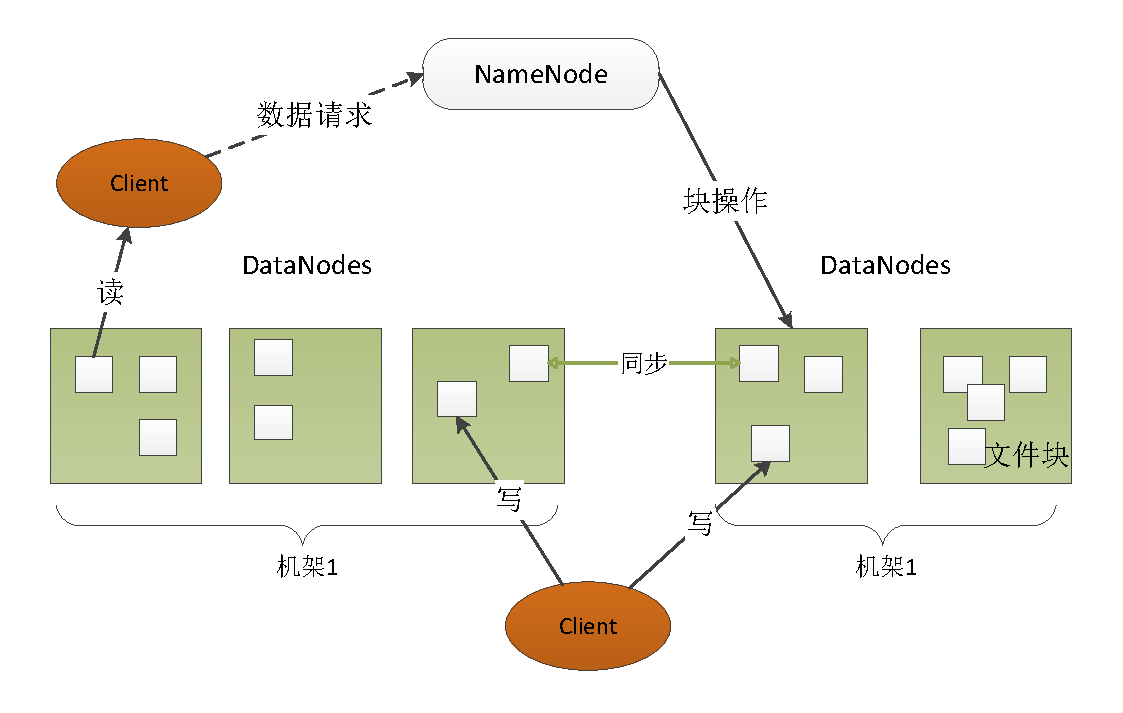
\includegraphics[width=1\textwidth]{HDFS架构}
 \caption{HDFS架构}
 \label{fig:HDFS架构}
\end{figure}

\begin{enumerate}
\item NameNode可以看作是分布式文件系统中的管理者,主要负责管理文件系统的命名空间、集群配置信息和存储块的复制等。NameNode会将文件系统的Meta-data存储在内存中,这些信息主要包括了文件信息、每一个文件对应的文件块的信息和每一个文件块在DataNode的信息等。
\item DataNode是文件存储的基本单元,它将Block存储在本地文件系统中,保存了Block的Meta-data,同时周期性地将所有存在的Block信息发送给NameNode。
\item Client就是需要获取分布式文件系统文件的应用程序。这里通过三个操作来说明他们之间的交互关系。
\end{enumerate}

文件写入:

\begin{enumerate}
\item Client向NameNode发起文件写入的请求。
\item NameNode根据文件大小和文件块配置情况,返回给Client它所管理部分DataNode的信息。
\item Client将文件划分为多个Block,根据DataNode的地址信息,按顺序写入到每一个DataNode块中。
\end{enumerate}

文件读取:

\begin{enumerate}
\item Client向NameNode发起文件读取的请求。
\item NameNode返回文件存储的DataNode的信息。
\item Client读取文件信息。
\end{enumerate}

文件Block复制:

\begin{enumerate}
\item NameNode发现部分文件的Block不符合最小复制数或者部分DataNode失效。
\item 通知DataNode相互复制Block。
\item DataNode开始直接相互复制。
\end{enumerate}

因此,HDFS具有以下的几个设计特点:

\begin{enumerate}
\item Block的放置:默认不配置。一个Block会有三份备份,一份放在NameNode指定的DataNode,另一份放在与指定DataNode非同一Rack上的DataNode,最后一份放在与指定DataNode同一Rack上的DataNode上。备份无非就是为了数据安全,考虑同一Rack的失败情况以及不同Rack之间数据拷贝性能问题就采用这种配置方式。
\item 心跳检测DataNode的健康状况,如果发现问题就采取数据备份的方式来保证数据的安全性。
\item 数据复制(场景为DataNode失败、需要平衡DataNode的存储利用率和需要平衡DataNode数据交互压力等情况):这里先说一下,使用HDFS的balancer命令,可以配置一个Threshold来平衡每一个DataNode磁盘利用率。例如设置了Threshold为10%,那么执行balancer命令的时候,首先统计所有DataNode的磁盘利用率的均值,然后判断如果某一个DataNode的磁盘利用率超过这个均值Threshold以上,那么将会把这个DataNode的block转移到磁盘利用率低的DataNode,这对于新节点的加入来说十分有用。
\item 数据交验:采用CRC32作数据交验。在文件Block写入的时候除了写入数据还会写入交验信息,在读取的时候需要交验后再读入。
\item NameNode是单点:如果失败的话,任务处理信息将会纪录在本地文件系统和远端的文件系统中。
\item 数据管道性的写入:当客户端要写入文件到DataNode上,首先客户端读取一个Block然后写到第一个DataNode上,然后由第一个DataNode传递到备份的DataNode上,一直到所有需要写入这个Block的NataNode都成功写入,客户端才会继续开始写下一个Block。
\item 安全模式:在分布式文件系统启动的时候,开始的时候会有安全模式,当分布式文件系统处于安全模式的情况下,文件系统中的内容不允许修改也不允许删除,直到安全模式结束。安全模式主要是为了系统启动的时候检查各个DataNode上数据块的有效性,同时根据策略必要的复制或者删除部分数据块。运行期通过命令也可以进入安全模式。在实践过程中,系统启动的时候去修改和删除文件也会有安全模式不允许修改的出错提示,只需要等待一会儿即可。
\end{enumerate}

HDFS是MapReduce的读写的底层实现,对MapReduce进化起着至关重要的作用。

\subsection[Hadoop的运行过程]{Hadoop的运行过程\cite{book:Hadoop}}
在Hadoop的系统中,会有一台Master,主要负责NameNode的工作以及JobTracker的工作。JobTracker的主要职责就是启动、跟踪和调度各个Slave的任务执行。还会有多台Slave,每一台Slave通常具有DataNode的功能并负责TaskTracker的工作。TaskTracker根据应用要求来结合本地数据执行Map任务以及Reduce任务。

具体如图\ref{fig:Hadoop运行流程}所示,过程如下:

\begin{enumerate}
\item 在分布式环境中客户端创建任务并提交。

\item InputFormat做Map前的预处理,主要负责以下工作:

1)验证输入的格式是否符合JobConfig的输入定义,这个在实现Map和构建Conf的时候就会知道,不定义可以是Writable的任意子类。

2)将input的文件切分为逻辑上的输入InputSplit,其实这就是在上面提到的在分布式文件系统中blocksize是有大小限制的,因此大文件会被划分为多个block。

3)通过RecordReader来再次处理inputsplit为一组records,输出给Map。inputsplit只是逻辑切分的第一步,但是如何根据文件中的信息来切分还需要RecordReader来实现,例如最简单的默认方式就是回车换行的切分。

\item RecordReader处理后的结果作为Map的输入,Map执行定义的Map逻辑,输出处理后的key和value对应到临时中间文件。

\item Combiner可选择配置,主要作用是在每一个Map执行完分析以后,在本地优先作Reduce的工作,减少在Reduce过程中的数据传输量。

\item Partitioner可选择配置,主要作用是在多个Reduce的情况下,指定Map的结果由某一个Reduce处理,每一个Reduce都会有单独的输出文件。(后面的代码实例中有介绍使用场景)

\item Reduce执行具体的业务逻辑,并且将处理结果输出给OutputFormat。

\item OutputFormat的职责是,验证输出目录是否已经存在,同时验证输出结果类型是否如Config中配置,最后输出Reduce汇总后的结果。
\end{enumerate}

\begin{figure}
 \centering
 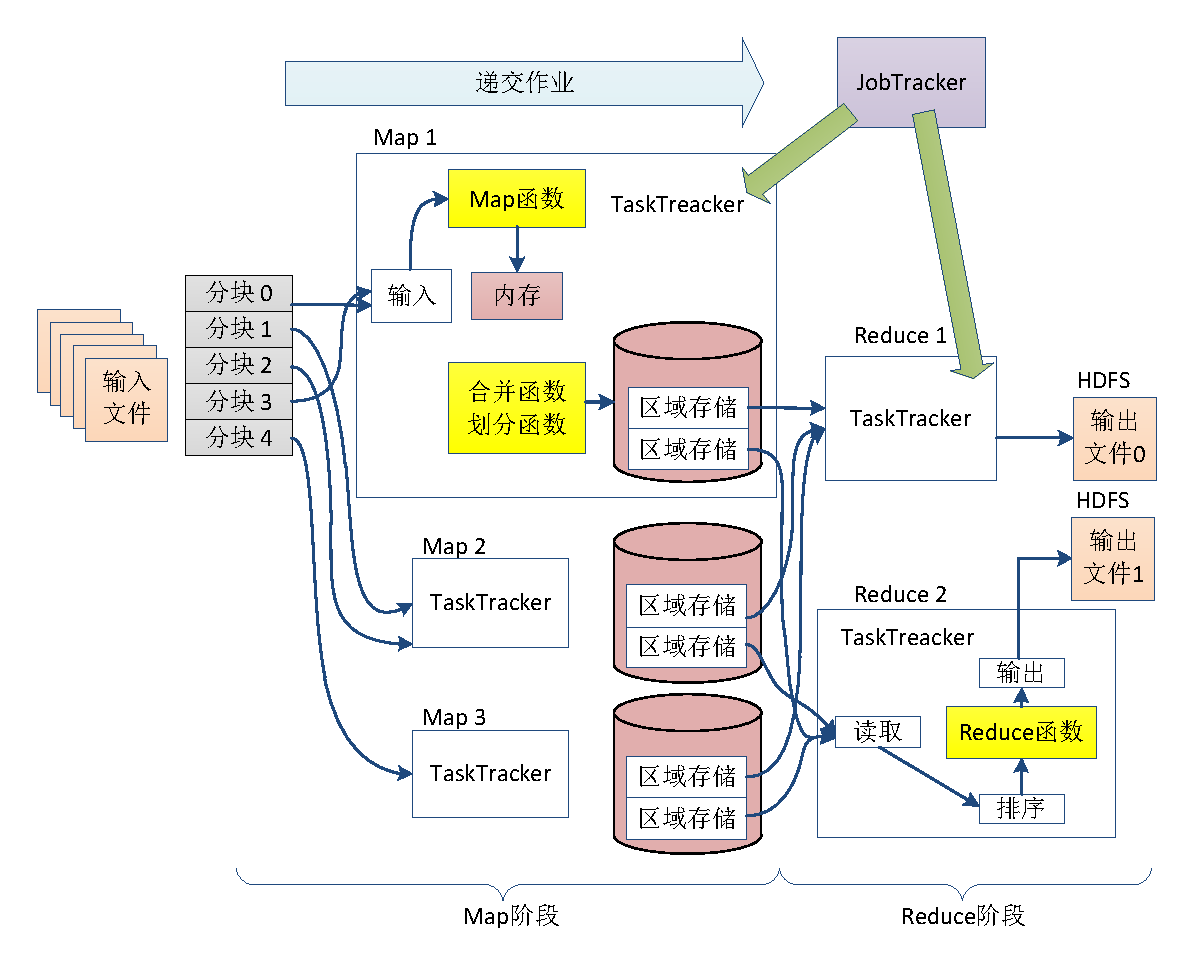
\includegraphics[width=1\textwidth]{Hadoop运行流程}
 \caption{Hadoop运行流程}
 \label{fig:Hadoop运行流程}
\end{figure}

\subsection{Hadoop的组成}
Hadoop整体功能由五个子进程实现,他们分别为NameNode、SecondaryNameNode、Jobtracker、DataNode和TaskTracker,其具体功能如下:

NameNode,NameNode是分布式文件系统的管理者,主要负责文件系统的命名空间,集群的配置信息和数据块的复制信息等,并将文件系统的元数据存储在内存中。

SecondaryNameNode,SecondaryNameNode有两个作用,一是镜像备份,二是日志与镜像的定期合并。它会周期性的将EditLog中记录的对HDFS的操作合并到一个checkpoint中,然后清空EditLog。如果没有SecondaryNameNode的这个周期性的合并过程,那么当每次重启NameNode的时候,就会花费很长的时间。而这样周期性的合并就能减少重启的时间。同时也能保证HDFS系统的完整性。

JobTracker,负责任务的接受初始化,调度以及对TaskTrackee的监控。JobTracker作为一个单独的JVM运行,对整个MapReduce程序的运行起着至关重要的作用。

DataNode,负责为响应来自HDFS客户机的读写请求。它们还响应创建、删除和复制来自NameNode的块的命令。并与NameNode通过心跳包来维持联系。DataNode,负责为响应来自是文件实际存储的位置,它将块(Block)的元数据信息存储在本地文件系统中,周期性地将所有的Block信息发给NameNode。

TaskTrackee,运行作业划分后的任务。

其中NameNode、SecondaryNameNode和Jobtracker运行在Master节点上,DataNode和TaskTracker运行在Slave节点上。

本文中,因为实验环境限制,Hadoop运行模式为伪分布式,即五个子进程均处于同一宿主机上。如图\ref{fig:五个子进程}

\begin{figure}[h]
 \centering
 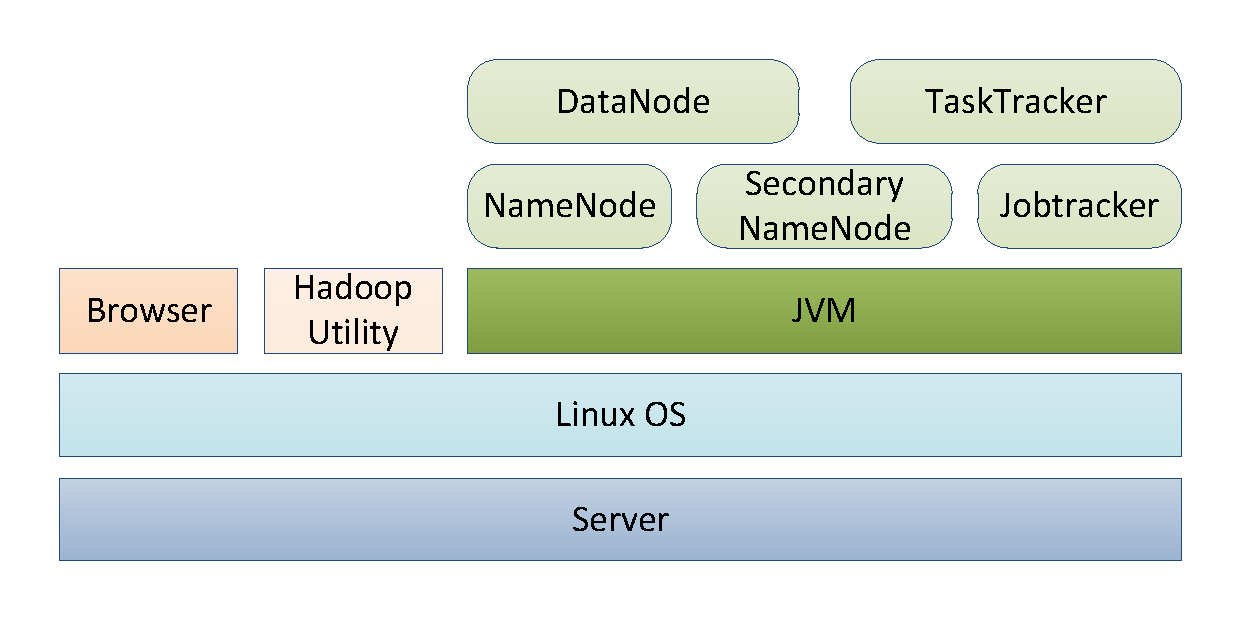
\includegraphics[width=0.9\textwidth]{五个子进程}
 \caption{五个子进程}
 \label{fig:五个子进程}
\end{figure}
%Hadoop基于SSH协议管理集群,节点间通过HDFS传输文件,程序运行时,Hadoop中的JobTracker守护进程负责调度节点,将Map和Reduce按照一定的规则分发到节点上的TaskTracker进程中,TaskTracker进程根据编写好的Map函数和Reduce函数从HDFS上获取数据并对其做进一步的处理。

%Mapper将HDFS中的文件按照事先编写好的Map函数进行处理,并将处理结果以Key/Value对的形式输出,之后,Hadoop会把Map结果根据键值合并,并将合并结果分发到集群用Reduce函数处理。这个过程中的整体通信会带来很大的网络I/O开销,尤其是在Map的开始和结束的时候,会带来一场大的“网络风暴”。同时,Hadoop会在运行时产生临时文件,从而带来很大的内存和磁盘开销。

%因此,运行Hadoop的机器应具有网络吞吐量好,可用内存大,磁盘读写速度快三个特点。

\subsection{Hadoop的特点}
Hadoop是面向大型集群实现MapReduce方法而设计的编程框架,其实现具有以下几个特点。

\begin{enumerate}
\item 可扩展:不论是存储的可扩展还是计算的可扩展都是Hadoop的设计根本。Hadoop中许多组件都是可插拔的,如调度器

\item 经济:框架可以运行在任何普通的PC上,使用者只需使用普通的PC机即可搭建性能强大的集群。

\item 可靠:分布式文件系统的备份恢复机制以及MapReduce的任务监控保证了分布式处理的可靠性。

\item 高效:分布式文件系统的高效数据交互实现以及MapReduce结合Local Data处理的模式,为高效处理海量的信息作了基础准备。

\item 使用方便:Hadoop使用Java语言实现,利用ssh协议与各节点之间通信,底层依赖小,可移植性强,适应于各种环境。
\end{enumerate}

\subsection{MapReduce在Hadoop中的三种实现方式及特点}

1. 原生Java
Hadoop是用Java编写的,所有Hadoop文件系统间的相互作用都是由Java API调解的。 举个例子,文件系统的shell就是一个Java应用,它使用Java文件系统类来提供文件系统操作。

同时,Hadoop提供了一套完整的Java类,用以实现MapReduce、HDFS操作及Hadoop配置。实际开发过程中,开发者可以直接引用这些类,达到快速开发的目的。

2. Streaming
Streaming框架允许任何程序语言实现的程序在Hadoop MapReduce中使用,方便已有程序向Hadoop平台移植。其原理是用Java实现一个包装用户程序的MapReduce程序,该程序负责调用MapReduce Java接口获取key/value对输入,创建一个新的进程启动包装的用户程序,将数据通过管道传递给包装的用户程序处理,然后调用MapReduce Java接口将用户程序的输出切分成key/value对输出。

Streaming天生适合用于文本处理(到0.21.0版本时,Streaming也可以处理二进制流),在文本模式下使用时,它有一个数据的行视图。map的输入数据通过标准输入流传递给map函数,并且是一行一行地传输,最后将结果行写到标准输出。map输出的键/值对是以一个制表符分隔的行,它以这样的形式写到标准输出。reduce 函数的输入格式相同——通过制表符来分隔的键/值对——并通过标准输入流进行传输。reduce函数从标准输入流中读取输入行,该输入已由Hadoop框架根据键排过序,最后将结果写入标准输出。

Streaming和Java MapReduce API在设计时有一些差异:Java API控制的map函数一次只能处理一条记录。针对输入数据中的每一条记录,该框架均需调用Mapper的map()方法来处理,然而在Streaming中,map程序可以自己决定如何处理输入数据,例如,它可以轻松读取并同时处理若干行,因为它受读操作的控制。用户的Java map实现的是“推”记录方式,但它依旧可以同时处理多行,具体做法是通过mapper中实例变量将之前读取的多行汇聚在一起。在这种情况下,需要实现close()方法,以便知道何时读到最后一条记录,进而完成对最后一组记录行的处理。

如下图\ref{fig:Streaming}所示,其中Streaming Java Mapper通过管道将key/value输入传递给用户mapper程序的标准输入,并获取用户mapper程序的标准输出;Streaming Java Reducer调用Java接口通过InputFormat从HDFS获取输入数据,从管道将key/value传递给用户 reducer程序的标准输入,获取用户reducer程序的标准输出并调用Java接口通过OutputFormat输出数据;用户mapper和reducer程序负责处理数据,都从标准输入读取数据,向标准输出写入数据。


\begin{figure}[h]
 \centering
 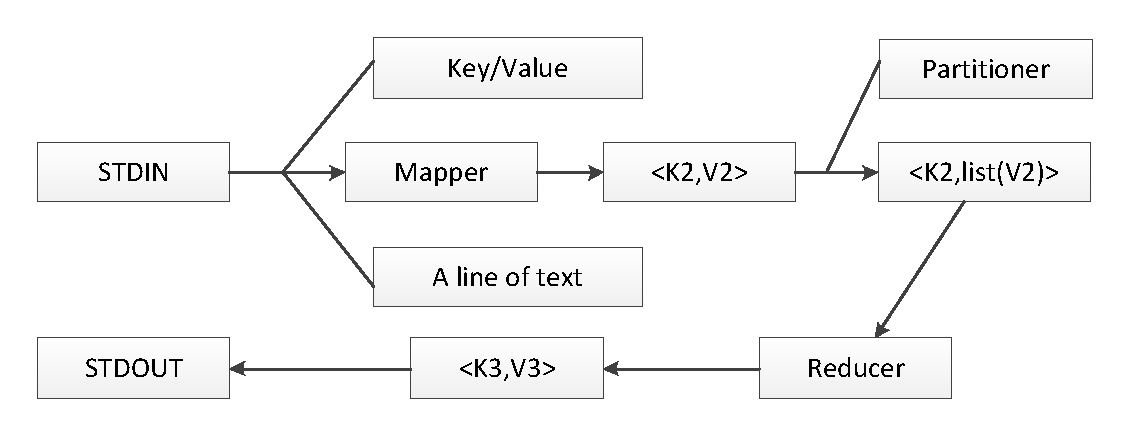
\includegraphics[width=1\textwidth]{Streaming}
 \caption{Streaming}
 \label{fig:Streaming}
\end{figure}


Streaming有如下一些优点: 

\begin{enumerate}
\item 开发效率高,很多现有程序(包括脚本)能够方便的移植到hadoop平台上去运行 

\item 某些程序运行效率高,对于某些cpu密集型程序,如果map-reduce程序用C++编写,效率有可能提高 
\end{enumerate}

Streaming存在如下一些不足:

\begin{enumerate}
\item Streaming中的mapper和reducer默认只能向标准输出写数据,不能方便地处理多路输出。 

\item 用Java编写的MapReduce程序直接处理框架从输入数据中得到的key/value对,在Streaming中Java程序不直接处理key/value对,而是通过管道写到mapper程序的标准输入,mapper程序再从key/tvalue中解析出key/value对,这个过程多了两次数据拷贝和解析(分割),带来一定的开销。对于reducer也是一样的。
\end{enumerate}

3. Pipes

Hadoop的Pipes是Hadoop MapReduce的C++接口代称。不同于使用标准输入和输出来实现map代码和reduce代码之间的Streaming,Pipes使用套接字作为tasktracker与C++版本map函数或reduce函数的进程之间的通道。

应用程序对Hadoop C++库链接提供了一个与tasktracker 子进程进行通信的简单封装。通过扩展HadoopPipes命名空间中定义的mapper和reducer两个类,我们定义了map()和reduce()方法,同时我们提供各种情况下map()和reduce()方法的实现。这些方法采用了上下文对象(MapContext类型或ReduceContext类型),进而提供了读取输入数据和写入输出数据,以及通过JobConf类来访问作业配置信息的功能。

与Java接口不同,C++接口中的键和值按字节缓冲,用标准模板库(Standard Template Library,STL)中的字符串表示。这样做简化了接口,但把更重的负担留给了应用程序开发人员,因为开发人员必须来回封送(marshall)字符串与特定应用领域内使用的具体类型。

因Pipes通过trasktracker子进程进行通信,但由于Hadoop提供的C++接口功能过于简单,开发负担大,故本文中仅对原生Java和Streaming的实现做性能对比。

\subsection[Hadooop计数器及其含义]{Hadooop计数器及其含义\cite{site:hadoop-counter}}
Hadoop里有一个很常用的工具叫计数器(Counter), 主要用来记录Hadoop job的运行状态。通过计数器,用户可以观察MapReduce job运行期间的各个细节数据,大多数优化都是基于计数器的数值表现。本文中后期的性能分析主要依靠Hadoop计数器提供的数据完成。

Hadoop job提供的默认计数器分为五个组分别是Job Counters、File Input Format Counters、File Output Format Counters、FileSystem Counters和Map-Reduce Framework其包含的数据和含义如下:

\begin{enumerate}

\item Job Counters 

这个计数器描述与job调度相关的统计 

Data-local map tasks:Job在被调度时,如果启动了一个data-local(源文件的幅本在执行map task的taskTracker本地) 

FALLOW\_SLOTS\_MILLIS\_MAPS:当前job为某些map task的执行保留了slot,总共保留的时间是多少 

FALLOW\_SLOTS\_MILLIS\_REDUCES:与上面类似 

SLOTS\_MILLIS\_MAPS:所有map task占用slot的总时间,包含执行时间和创建/销毁子JVM的时间 

SLOTS\_MILLIS\_REDUCES:与上面类似 

Launched map tasks:此job启动了多少个map task 

Launched reduce tasks:此job启动了多少个reduce task 


\item File Inut Format Counters

这个计数器表示map task读取文件内容(总输入数据)的统计

BYTES\_READ:Map task的所有输入数据(字节),等于各个map task的map方法传入的所有value值字节之和。 

\item File Output Format Counters

这个计数器表示map task写入文件内容(总输入数据)的统计

BYTES\_READ:Map task的所有输出数据(字节),等于各个map task的map方法传出的所有value值字节之和。 

\item FileSystem Counters

MapReduce job执行所依赖的数据来自于不同的文件系统,这个计数器表示job与文件系统交互的读写统计 

FILE\_BYTES\_READ:job读取本地文件系统的文件字节数。假定我们当前map的输入数据都来自于HDFS,那么在map阶段,这个数据应该是0。但reduce在执行前,它的输入数据是经过shuffle的merge后存储在reduce端本地磁盘中,所以这个数据就是所有reduce的总输入字节数。 

FILE\_BYTES\_WRITTEN:map的中间结果都会spill到本地磁盘中,在map执行完后,形成最终的spill文件。所以map端这里的数据就表示map task往本地磁盘中总共写了多少字节。与map端相对应的是,reduce端在shuffle时,会不断地拉取map端的中间结果,然后做merge并不断spill到自己的本地磁盘中。最终形成一个单独文件,这个文件就是reduce的输入文件。 

HDFS\_BYTES\_READ:整个job执行过程中,只有map端运行时,才从HDFS读取数据,这些数据不限于源文件内容,还包括所有map的split元数据。所以这个值应该比FileInputFormatCounters.BYTES\_READ 要略大些。 

HDFS\_BYTES\_WRITTEN:Reduce的最终结果都会写入HDFS,就是一个job执行结果的总量。 


\item Map-Reduce Framework

这个计数器包含了相当多地job执行细节数据。这里需要有个概念认识是:一般情况下,record就表示一行数据,而相对地byte表示这行数据的大小是多少,这里的计数器表示经过reduce merge后像这样的输入形式{“aaa”, [5, 8, 2, …]}。 

Combine input records:Combiner是为了减少尽量减少需要拉取和移动的数据,所以combine输入条数与map的输出条数是一致的。 

Combine output records:经过Combiner后,相同key的数据经过压缩,在map端自己解决了很多重复数据,表示最终在map端中间文件中的所有条目数 

Failed Shuffles:copy线程在抓取map端中间数据时,如果因为网络连接异常或是IO异常,所引起的shuffle错误次数 

GC time elapsed(ms):通过JMX获取到执行map与reduce的子JVM总共的GC时间消耗 

Map input records:所有map task从HDFS读取的文件总行数 

Map output records:map task的直接输出record是多少,就是在map方法中调用context.write的次数,也就是未经过Combine时的原生输出条数 

Map output bytes:Map的输出结果key/value都会被序列化到内存缓冲区中,所以这里的bytes指序列化后的最终字节之和 

Merged Map outputs:记录着shuffle过程中总共经历了多少次merge动作 

Reduce input groups:Reduce总共读取了多少个这样的计数器 

Reduce input records:如果有Combiner的话,那么这里的数值就等于map端Combiner运算后的最后条数,如果没有,那么就应该等于map的输出条数 

Reduce output records:所有reduce执行后输出的总条目数 

Reduce shuffle bytes:Reduce端的copy线程总共从map端抓取了多少的中间数据,表示各个map task最终的中间文件总和 

Shuffled Maps:每个reduce几乎都得从所有map端拉取数据,每个copy线程拉取成功一个map的数据,那么增1,所以它的总数基本等于 reduce number * map number 

Spilled Records:spill过程在map和reduce端都会发生,这里统计在总共从内存往磁盘中spill了多少条数据 

SPLIT\_RAW\_BYTES 
与map task 的split相关的数据都会保存于HDFS中,而在保存时元数据也相应地存储着数据是以怎样的压缩方式放入的,它的具体类型是什么,这些额外的数据是MapReduce框架加入的,与job无关,这里记录的大小就是表示额外信息的字节大小 

\end{enumerate}
	
	
\section[Web访问日志简介]{Web访问日志简介\cite{site:weblog}}
\subsection{什么是Web访问日志}
Web访问日志是Web服务器的运行记录文档,当用户访问一个网站时,服务器上的Web服务会接受该用户的请求,并将用户的请求信息记录并保存下来。目前常见的Web访问日志格式主要由两类,一类是Apache的NCSA日志格式,另一类是IIS的W3C日志格式。NCSA格式又分为NCSA普通日志格式(CLF)和NCSA扩展日志格式(ECLF)两类,目前最常用的是NCSA扩展日志格式(ECLF)及基于自定义类型的Apache日志格式;而W3C扩展日志格式(ExLF)具备了更为丰富的输出信息,但目前的应用并不广泛。目前,大多数网站使用NCSA日志格式来存储日志。

Nginx是一款基于Epoll模型的web服务程序\cite{site:nginx},近年来发展迅猛,截止2012年5月,Nginx已经占据Web软件10.32\%的份额\cite{site:netcraft_nginx},Nginx的默认日志为Apache的NCSA扩展日志格式(ECLF),本实验中所用的日志为Nginx默认生成的日志。

\subsection{NCSA扩展日志格式的组成}
这是一个最常见的基于NCSA扩展日志格式(ECLF)的Nginx日志样例:

\begin{verbatim}
222.25.151.30 - - [28/May/2012:19:12:03 +0800] "GET /bbs/uc_server/ava
tar.php?uid=46369&size=small HTTP/1.1" 301 0 "http://rs.xidian.edu.cn/
bbs/index.php" "Mozilla/4.0 (compatible; MSIE 8.0; Windows NT 5.1; Tri
dent/4.0; GTB7.2; .NET CLR 1.1.4322; .NET CLR 2.0.50727; CIBA; TheWorl
d)" -
\end{verbatim}

可以很清楚的看到,这个日志主要由以下几个部分组成:

\begin{enumerate}
\item 访问主机(remotehost)

显示主机的IP地址或者已解析的域名。

\item 标识符(Ident)

由identd或直接由浏览器返回浏览者的EMAIL或其他唯一标示,因为涉及用户邮箱等隐私信息,目前几乎所有的浏览器就取消了这项功能。

\item 授权用户(authuser)

用于记录浏览者进行身份验证时提供的名字,如果需要身份验证或者访问密码保护的信息则这项不为空,但目前大多数网站的日志这项也都是为空的。

\item 日期时间(date)

一般的格式形如[22/Feb/2010:09:51:46 +0800],即[日期/月份/年份:小时:分钟:秒钟 时区],占用的的字符位数也基本固定。

\item 请求(request)

即在网站上通过何种方式获取了哪些信息,也是日志中较为重要的一项,主要包括以下三个部分:


\item 请求类型(METHOD)

常见的请求类型主要包括GET/POST/HEAD这三种;


\item 请求资源(RESOURCE)


显示的是相应资源的URL,可以是某个网页的地址,也可以是网页上调用的图片、动画、CSS等资源,是Web访问日志挖掘中的一个重点;


\item 协议版本号(PROTOCOL)


显示协议及版本信息,通常是HTTP/1.1或HTTP/1.0。

\item 状态码(status)

用于表示服务器的响应状态,通常1xx的状态码表示继续消息;2xx表示请求成功;3xx表示请求的重定向;4xx表示客户端错误;5xx表示服务器错误。

\item 传输字节数(bytes)

即该次请求中一共传输的字节数。

\item 来源页面(referrer)

用于表示浏览者在访问该页面之前所浏览的页面,只有从上一页面链接过来的请求才会有该项输出,如果是新开的页面则该项为空。上例中来源页面是google,即用户从google搜索的结果中点击进入。

\item 用户代理(agent)

用于显示用户的详细信息,包括IP、OS、Bowser等。

\end{enumerate}

\subsection{Web访问日志的作用及价值}
Web访问日志记录了用户访问一个网站的所有过程,是个非常好的数据挖掘原料。通过对Web访问日志的分析,网站服务提供商可以获得某一指定用户的点击流(Clickstream),网站的流量及访问时段,网站的内部漏洞及可能的注入点。

有效的利用Web访问日志可以高效精准的分析出用户喜好,帮助网站运营商提升网站质量。

\section{本章小结}
本章主要介绍本文的研究背景,详述了MapReduce、Hadoop的起源、发展及其运行机制,并详述了Hadoop Counter和Web访问日志的内容及其格式。为进一步的开发和研究做了铺垫。